\documentclass[
letterpaper,
11pt,
answers,
]{exam}

\usepackage[lmargin=0.75in,rmargin=0.75in,tmargin=1in,bmargin=1in]{geometry}
\usepackage{soul}
\usepackage{enumitem}
\usepackage{graphicx}
\usepackage{tikz}
\usepackage{multicol}
\usepackage[randomize]{exam-randomizechoices}
\setrandomizerseed{28056}

% Sets the column separation so that enumeration doesn't cause
% the line between columns interfere with the numbers.
\setlength{\columnsep}{4em}
%\setlength{\columnseprule}{0.4pt}

% Code block creates the Matching question format
\newcommand*\Matching[1]{
\ifprintanswers
\textbf{#1}
\else
\rule{2.5in}{0.5pt}
\fi
}
\newlength\matchlena
\newlength\matchlenb
\settowidth\matchlena{\rule{2.5in}{0pt}}
\newcommand\MatchQuestion[2]{%
\setlength\matchlenb{\linewidth}
\addtolength\matchlenb{-\matchlena}
\parbox[t]{\matchlena}{\Matching{#1}}\enspace\parbox[t]{\matchlenb}{#2}}

% Formats the header on the first page where the student enters their name and date.
\newcommand{\head}{%
\thispagestyle{empty}
\vspace*{-0.75in}
\noindent
\class \hfill Name \makebox[7cm]{\hrulefill} Ver: \wsVer\par
\vspace{10pt}
\noindent
\Large\textbf{\wstitle}\normalsize \hfill Date \makebox[3.5cm]{\hrulefill}\par
\vspace{10pt}
}

% Defines the titles and instructions for the worksheet or test
\newcommand{\class}{Humanities}
\newcommand{\wstitle}{\textit{Template} Test}
\newcommand{\wsVer}{1}
\newcommand{\Instructions}{Fill in each blank with the name corresponding to the number on the map.}

% Sets the running header at the top of the subsequent pages
\pagestyle{head}
\runningheader{\class\ \wstitle}{}{Page \thepage\ of \numpages}

% BEGINNING OF DOCUMENT
\begin{document}
\head
\setlength{\linewidth}{6.5in}

% Display the map/image with the labels applied
\noindent
\begin{tikzpicture}
    % Include the image
    \node[anchor=south west,inner sep=0] at (0,0) {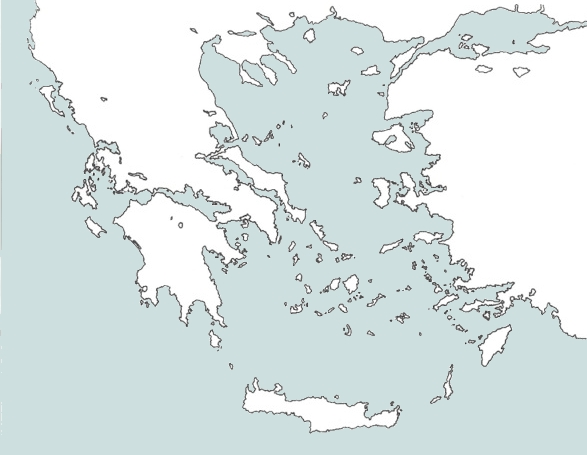
\includegraphics[width=\textwidth]{blankGreekmap.jpg}};

    % Overlay text at specific coordinates
    %\node at (1, 1) {\textbf{LABEL}};  % (1, 1) is location (in cm) of LABEL on the map/image
    \node at (2, 2) {\textbf{2,2}};
    \node at (3, 3) {\textbf{3,3}};
    \node at (4, 4) {\textbf{4,4}};
    \node at (5, 5) {\textbf{5,5}};
    \node at (6, 6) {\textbf{6,6}};
    \node at (7, 7) {\textbf{7,7}};
    \node at (8, 8) {\textbf{8,8}};
    \node at (9, 9) {\textbf{9,9}};
    \node at (10, 1.2) {\textbf{Crete}};
    \node at (11, 11) {\textbf{11,11}};
    \node at (12, 12) {\textbf{12,12}};
    \node at (13, 13) {\textbf{13,13}};
    \node at (14, 14) {\textbf{14,14}};
    \node at (15, 14) {\textbf{15,14}};
    \node at (16, 14) {\textbf{16,14}};
    \node at (17, 14) {\textbf{16,14}};
\end{tikzpicture}
%}

\noindent
\textit{\Instructions}\par
%\textit{Fill in each blank with the name corresponding to the number on the map.}\par

\begin{questions}

\begin{multicols}{2}
% \question\MatchQuestion{ANSWER}{PROMPT} \vfill
\question\MatchQuestion{A}{} \vfill
\question\MatchQuestion{Boeotia}{} \vfill
\question\MatchQuestion{Mycenaia}{} \vfill
\question\MatchQuestion{Troy}{} \vfill
\question\MatchQuestion{Olympia}{} \vfill
\question\MatchQuestion{Corinth}{} \vfill
\question\MatchQuestion{Sparta}{} \vfill
\end{multicols}

\end{questions}
\end{document}